

In contrast to section \vref{sec:extVel}, this section describes
motion using a internally generated velocity field.


\subsection{Motion in the normal direction}

One of the most simple things we can do, is to move the interface in
the normal direction $\vec{N}$ using a constant $a$, efficiently
scaling the iso-surface.

From equation \vref{velocity:levelseteq} we have:
\begin{equation}
  \phi_t + \vec{V}\cdot \nabla \phi = 0
\end{equation}
Since $a\vec{N}$ has the same direction as $\nabla{\phi}$, we have the following:
\begin{align*}
  a\vec{N}\cdot\nabla\phi &=
  a\frac{\nabla\phi}{|\nabla\phi|}\cdot\nabla\phi \\
  &= a\frac{|\nabla\phi|^2}{|\nabla\phi|} 
  = a|\nabla\phi|
\end{align*}

With corresponds to this level set equation:

\begin{equation}
  \phi_t + a |\nabla \phi| = 0
\end{equation}\label{eq:lsgrow}

At this point, the point of the signed distances field is clear, if
$\phi$ is a SDF, then $|\nabla\phi| = 1$. This means that we can solve
(\ref{eq:lsgrow}) very simply using the forward euler method (see
equation \ref{eq:fweuler}).

This corresponds to the following code:

\begin{lstlisting}
for(unsigned int x=0; x<width; x++) {
    for(unsigned int y=0; y<height; y++) {
        phi(x,y) += -a;
    }
}
\end{lstlisting}

A sample is shown in figure \ref{fig:auGrow} where the AU logo is
expanded with $a=1.0$ for 6 and 20 iterations.


\begin{figure}[h]
  \centering
  \subfloat[The original logo]{
    
\includegraphics[width=0.3\textwidth]{imgs/au-logo}
    \label{fig:au}
  }
  \subfloat[After 6 iterations]{
    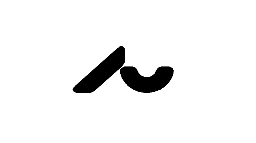
\includegraphics[width=0.3\textwidth]{imgs/auGrow6}}
  \subfloat[After 20 iterations]{
    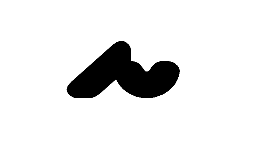
\includegraphics[width=0.3\textwidth]{imgs/auGrow20}}
  \caption{The AU logo after expanding with $a=1.0$ for 6 and 20 iterations}
  \label{fig:auGrow}
\end{figure}


\subsection{Mean-Curvature}

Another interesting thing we can do with a level set, is to move the
interface in the normal direction with a velocity proportional to its
curvature (this is called mean-curvature). The effect of this is to
soften or sharpen the interface.

To do this we need the following velocity field:
\begin{equation}
  \vec{V} = -b\kappa\vec{N}
\end{equation}

Where $\kappa$ is the curvature, and $b>0$ is a constant describing the
speed of the motion. % \todoPtx{Explain why $b>0$?}

This corresponds to the level set equation: 
\begin{equation}
  \phi_t -b\kappa|\nabla\phi| = 0
\end{equation}

This is a parabolic equation, so to discretize it we need to use a new
approach. 

We start by exploring the curvature $\kappa$. It is defined as:
\begin{equation}
  \kappa = \nabla\cdot\left(\frac{\nabla\phi}{|\nabla\phi|}\right)
\end{equation}

When $\phi$ is a SDF, then $|\nabla\phi|=1$, which simplifies our equation
to: $\kappa = \nabla^2\phi$. Which is the laplacian operator: $\kappa =
\Delta\phi$. In this context, $\Delta\phi$ is defined as:
\begin{equation}
  \Delta\phi = \phi_{xx} + \phi_{yy}
\end{equation}

$\phi_{xx}$ and $\phi_{yy}$ can be solved using central difference:
\begin{equation}
  D^+_xD^-_x\phi 
  % \frac{\partial^2\phi}{\partial x^2} % Should we use \partial or D?
  \approx
  \frac{\phi_{i+1}-2\phi_i+\phi_{i-1}}{\Delta x^2}
\end{equation} % eq 1.9 s. 12

Again the forward Euler method can be used, but we have to use a small
time step according to \citbook{osher2002level}{page~44}:
\begin{equation}
   \Delta t \left(
     \frac{2b}{(\Delta x)^2} +
     \frac{2b}{(\Delta y)^2}
   \right) < 1
\end{equation}

If we respect these, then the  implementation is straight forward:

% using formula 1.9 on page 12 and
% using formula 2.7 on page 21.
% using formula 4.11 on page 45

\begin{lstlisting}
for(unsigned int x=1; x<width-1; x++) {
    for(unsigned int y=1; y<height-1; y++) {
        const float dx = 1.0;
        float phi_xx = (phi(x+1,y) - 2*phi(x,y) + phi(x-1,y))/(dx*dx);
        float phi_yy = (phi(x,y+1) - 2*phi(x,y) + phi(x,y-1))/(dx*dx);

        float kappa = phi_xx + phi_yy;
        phi(x,y) += kappa * a; //mean curvature
    }
}
\end{lstlisting}

\begin{figure}[h]
  \centering
  \subfloat[The original logo]{
    
\includegraphics[width=0.3\textwidth]{imgs/au-logo}
  }
  \subfloat[After 20 iterations]{
    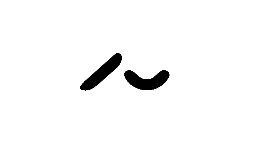
\includegraphics[width=0.3\textwidth]{imgs/auMean20}}
  \subfloat[After 100 iterations]{
    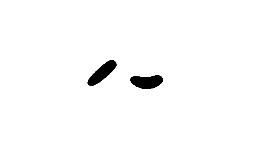
\includegraphics[width=0.3\textwidth]{imgs/auMean100}}
  \caption{The AU logo after mean-curvature with $a=0.4$ for 20 and 100 iterations}
  \label{fig:auMean}
\end{figure}



This is demonstrated in figure \ref{fig:auMean}. The logo becomes less
sharp, and if continued long enough, it will disappear. 



\subsection{Morph}
Another simple way of evolving the interface is a technique called
``morphing''. Given two signed distance fields, we can ``morph'' one
into the other simply by using the difference in fields in place of
velocity of change. This is a simple idea which can yield visually
impressive results.

The operation of morphing $\phi_1$ to $\phi_2$ is captured in this
equation:

\begin{align}
\phi_t = \phi_1 + (\phi_2 - \phi_1) \cdot -a
\end{align}


Figure \vref{fig:morph} shows the intuition behind the equation. The
parts of the field that are ``inside'' one curve and ``outside''
another yield higher differences than the parts that are inside or
outside both curves. Depending on the sign of $a$, the equation adds a
term to $\phi_1$ that increases or decreases its values in
correspondance to the difference of the fields. The result of this is
that the level sets of one field are evolved to resemble the curves of
the other.


\begin{figure}[h]
  \centering
  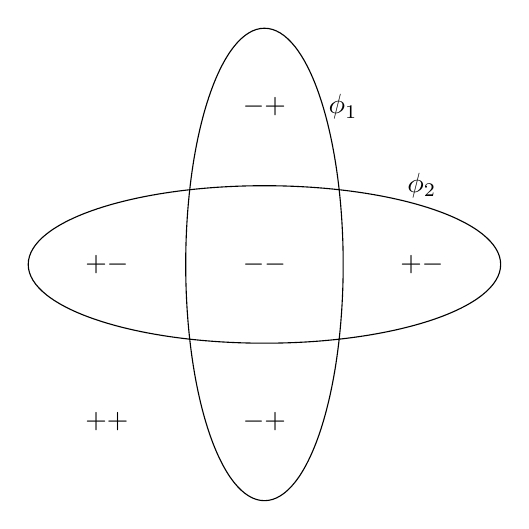
\begin{tikzpicture}
    \draw (0,0) ellipse (3cm and 1cm); \draw (0,0) ellipse (1cm and
    3cm); \draw (0,0) node {$--$}; \draw (2,0) node {$+-$}; \draw
    (-2,0) node {$+-$}; \draw (0,2) node {$-+$}; \draw (0,-2) node
    {$-+$}; \draw (-2,-2) node {$++$}; \draw (1,2) node {$\phi_1$};
    \draw (2,1) node {$\phi_2$};
  \end{tikzpicture}  
  \caption{Morphing two SDFs}
\label{fig:morph}
\end{figure}


The implementation is simply as follows:

\begin{lstlisting}
for(unsigned int x=0; x<width; x++) {
    for(unsigned int y=0; y<height; y++) {
        phi(x,y) += (phi(x,y) - phi2(x,y)) * -a; //morph
    }
}
\end{lstlisting}

% \subsection{CFG condition (Stability)}
% WTF is this?

%%% Local Variables: 
%%% mode: latex
%%% mode: auto-fill
%%% TeX-PDF-mode: t
%%% TeX-master: "../master.tex"
%%% End: 
